\begin{figure}[htbp]
\centering
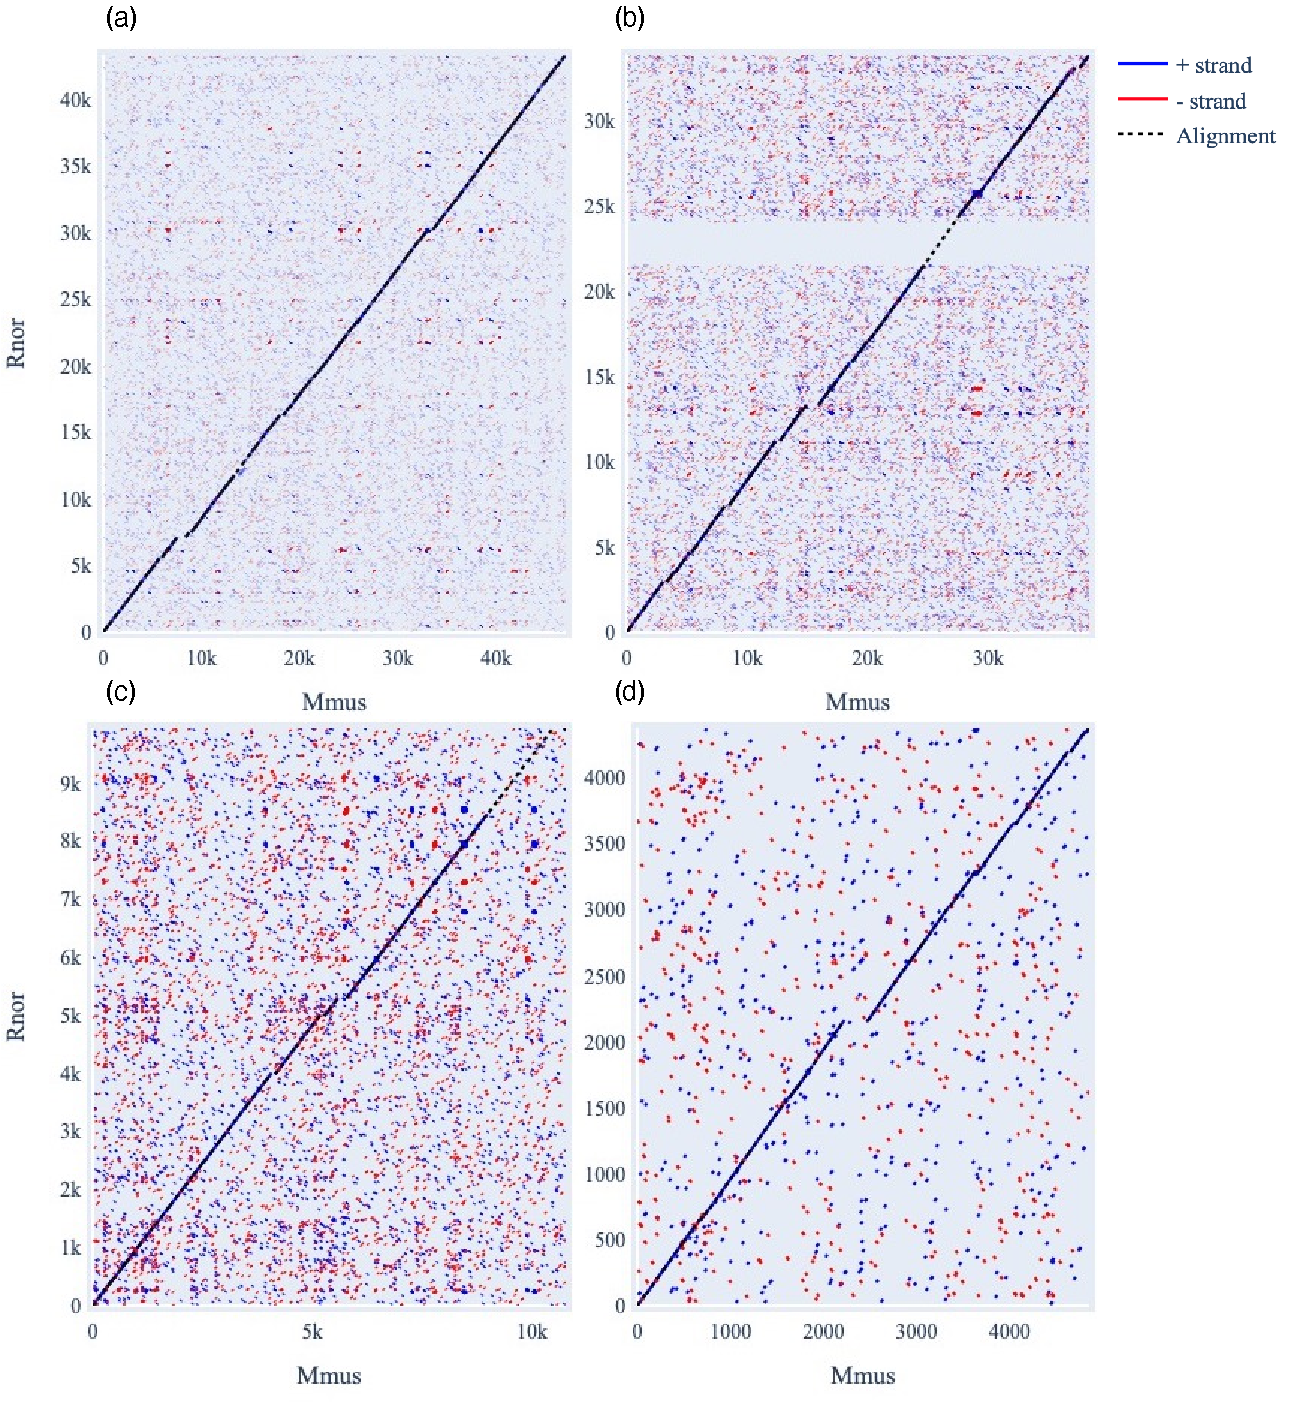
\includegraphics[width=\textwidth]{figures/diagrams/fxy_dotplot_1.pdf}
\caption[Dotplots of \textit{Fxy} introns 1-4]{ \textbf{Dotplots of \textit{Fxy} introns 1-4}. The alignment path between the sequences is shown as the dotted line. Long stretches of identity between sequences form a diagonal. The window was 20bp long, 20-mers identical at $>13$ positions were considered a match. The $x$- and $y$-axis are positions in the unaligned sequence.}
\label{fig:Fxy-dp-1}
\end{figure}